\section{Real Data}
\label{sec:data}

We analyzed a dataset that was collected to investigate the eating preferences of the wolf spider, genus \textit{Schizocosa}, towards the prey orders Diptera and Collembola.  Predators were collected in traps within the deciduous Berea College Forest in Madison County, Kentucky, USA and had their gut-contents analyzed to determine whether or not the spiders ate any Diptera or Collembola within each time period.  The left panel of figure~\ref{fig:data} plots the percentage of spiders that had the prey in their guts across time.  Prey were also collected in traps from the same area.  These data were collected for each month from October $2011$ to March $2013$.  On average, $69$ spiders, and $111$ and $297$ Diptera and Collembola, respectively, were caught in each time period.  The range of the sample sizes, across all $18$ months is, $11$ to $181$ for caught spiders, from $7$ to $322$ for trapped Diptera, and from $101$ to $755$ for trapped Collembola.  The right panel of figure~\ref{fig:data} plots the total number of each order that was caught during each time period. 

\begin{figure}
  \centering
  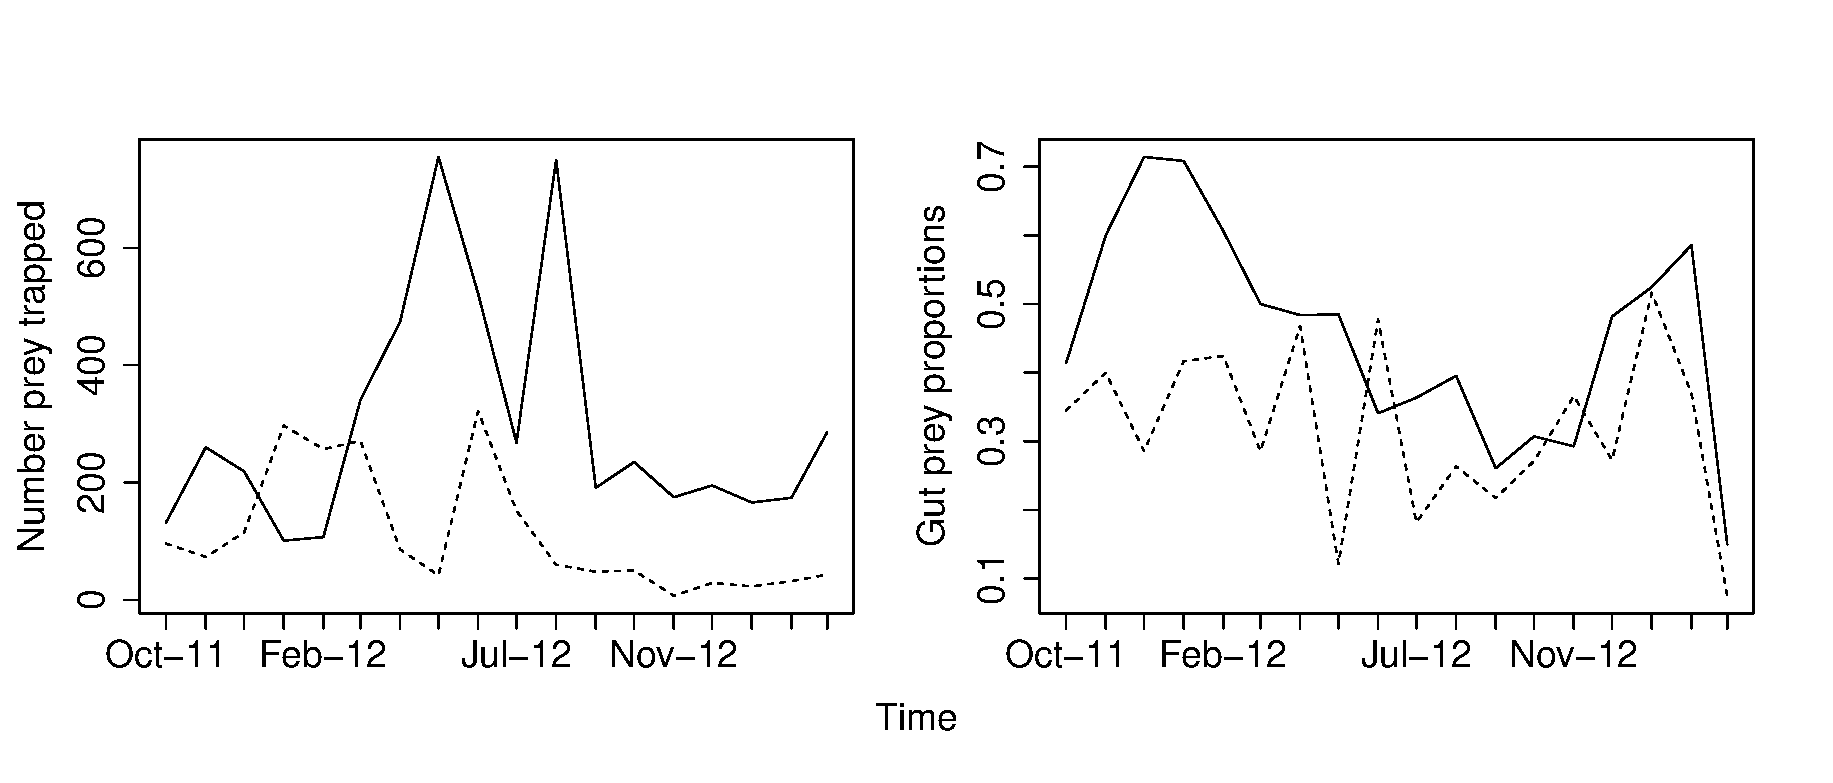
\includegraphics[scale=0.5]{data}
  \caption{For both Diptera and Collembola, the plots show the proportion of spiders with these orders found in their guts, and the number of these orders trapped in each time period.}
  \label{fig:data}
\end{figure}


These data provide an example of our hierarchy of hypotheses.  First, we tested model $c_{st} = c$ against $c_{st} = c_s$, to determine whether or not the wolf spider has different preferences for the two orders Diptera  and Collembola.  With, one degree of freedom, this likelihood ratio test indicated, $p-value < 0.0001$,  that two parameters, one for each order, fits these data better than one parameter for both.  Similarly, we tested whether or not there was a significant effect across time by testing model $c_{st} = c$ against $c_{st} = c_t$.  Here, the likelihood ratio test, with $17$ degrees of freedom, implies that the wolf spiders of the Berea College Forest eat these prey orders at different rates across the months of the year, $p-value < 0.0001$.  In fact, we find that the most parameter rich model, $\lambda_{st} = c_{st} \gamma_{st}$ fits these data better than is expected by chance, $p-value < 0.0001$.  Model $c_{st}$ estimates $72$ parameters in total; since, in this case, there are two prey of interest and $18$ time periods, it takes $36$ parameters to estimate each $c_{st}$ and $\gamma_{st}$.  Figure~\ref{fig:cst} plots the point estimates and $95\%$ confidence intervals of $c_{st}$, for both prey across all time periods.  

\begin{figure}
  \centering
  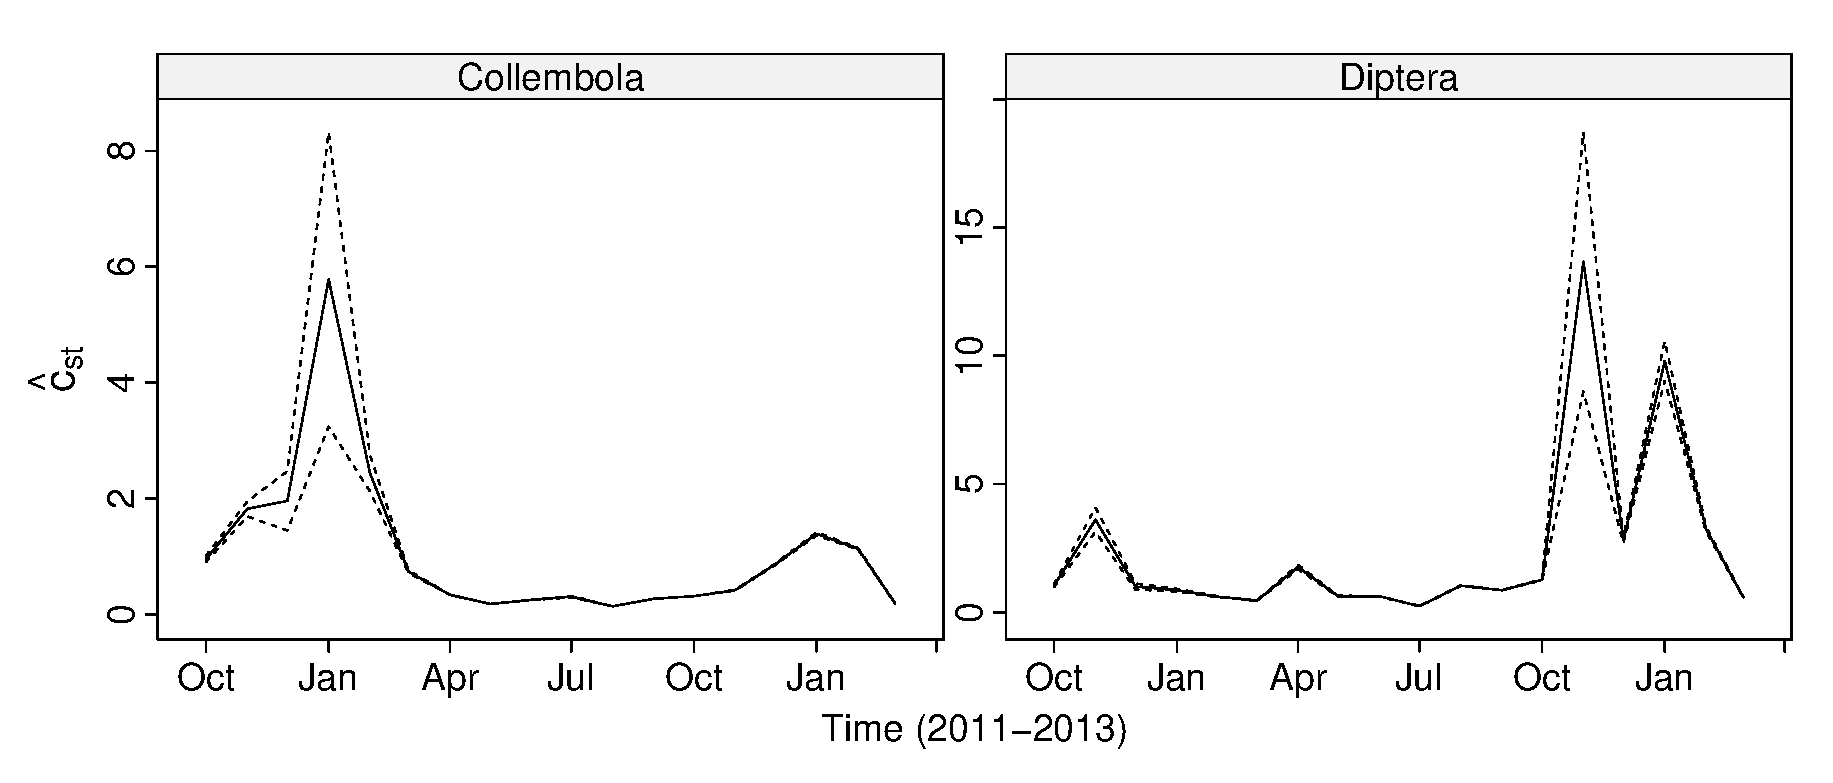
\includegraphics[scale=0.5]{cst}
  \caption{One plot for each prey order displays the point estimates and $95\%$ confidence intervals as estimated from the model $c_{st}$.}
  \label{fig:cst}
\end{figure}

With point estimates of $c_{st}$ under the model $\lambda_{st} = c_{st} \gamma_{st}$, we can test any number of linear contrasts.  For instance, $c_{1t} = c_{2t}$, for $t \in \{1, \ldots, 18\}$.  Using a level of significance of $0.05$, and after making a Bonferroni multiple comparisons adjustment, the data can not say that the two prey are differently preferred in October, November, and December of $2011$ and for March and July of $2012$.  


%%% Local Variables: 
%%% mode: latex
%%% TeX-master: "main"
%%% End: 
